\documentclass[11pt,twoside]{article} % use larger type; default would be 10pt

\usepackage{graphicx} % support the \includegraphics command and options
\usepackage{geometry} % See geometry.pdf to learn the layout options. There are lots.
\usepackage{gregoriotex} % for gregorio score inclusion
\usepackage{fullpage} % to reduce the margins
\usepackage[toc,page]{appendix}

\pdfminorversion=4

% choose the language of the document here
\usepackage[latin,frenchb]{babel}

% use the two following package for using normal TeX fonts
\usepackage[T1]{fontenc}
\usepackage[utf8]{luainputenc}

% If you use usual TeX fonts, here is a starting point:
\usepackage{times}

\usepackage{layout}

\usepackage{parallel}
\usepackage{color}
\usepackage{pdfcolmk}
\usepackage{xcolor}
\usepackage{fancyhdr}
\usepackage{txfonts}
\usepackage{textcomp}
\usepackage{yfonts}

\usepackage{fontspec}
\defaultfontfeatures{Mapping=tex-text}
\usepackage{libertine}

\usepackage{fullpage} % to reduce the margins
\setlength{\hoffset}{-1in}
\setlength{\voffset}{-1in}
\setlength{\paperwidth}{155mm}
\setlength{\textwidth}{130mm}
\setlength{\oddsidemargin}{\paperwidth * \real{0.5} - \textwidth * \real{0.5}}
\setlength{\evensidemargin}{\paperwidth * \real{0.5} - \textwidth * \real{0.5}}
\setlength{\paperheight}{219.17mm}
\setlength{\topmargin}{10.0mm}
\setlength{\textheight}{179.17mm}
\setlength{\footskip}{10.0mm}
\setlength{\marginparwidth}{0mm}
\setlength{\marginparsep}{0mm}
\mag=1355 % Pour revenir en 210mm x 297mm

\pagestyle{fancy}
\headheight=20pt
\headsep=15pt

\usepackage{float}
 
\floatstyle{plain}
\newfloat{piece}{H}

\input ../commun/commun.tex

\begin{document}
\fontsize{12.5}{13.5}\selectfont

% Debug : affichage des paramètres du layout
%\layout*

% Paramètrage des entètes
\fancyhead{} % clear all header fields
\fancyhead[CE]{\bfseries \uppercase{Office des Ténèbres}}
\fancyhead[CO]{\bfseries \uppercase{Samedi Saint}}
\fancyfoot{} % clear all footer fields
\fancyfoot[LE,RO]{\thepage}
\fancyfoot[CO,CE]{\small{Schola Saint-Maur}}
\renewcommand{\headrulewidth}{0.4pt}
\renewcommand{\footrulewidth}{0.4pt}

\def\greinitialformat#1{%
{\fontsize{33}{33}\selectfont #1}%
}

\def\grebiginitialformat#1{%
{\fontsize{33}{33}\selectfont #1}%
}

% Première page
\selectlanguage{francais}
\begin{titlepage}



\begingroup
\begin{center}
{\color{rougeliturgique}\Large \initfamily O}{\fontfamily{requi2}\fontsize{32}{12}\selectfont FFICE DES T\'EN\`EBRES}

\vspace{0.5cm}

{\fontfamily{requi2}\fontsize{22}{12}\selectfont DU SAMEDI SAINT}


\vspace*{2cm}

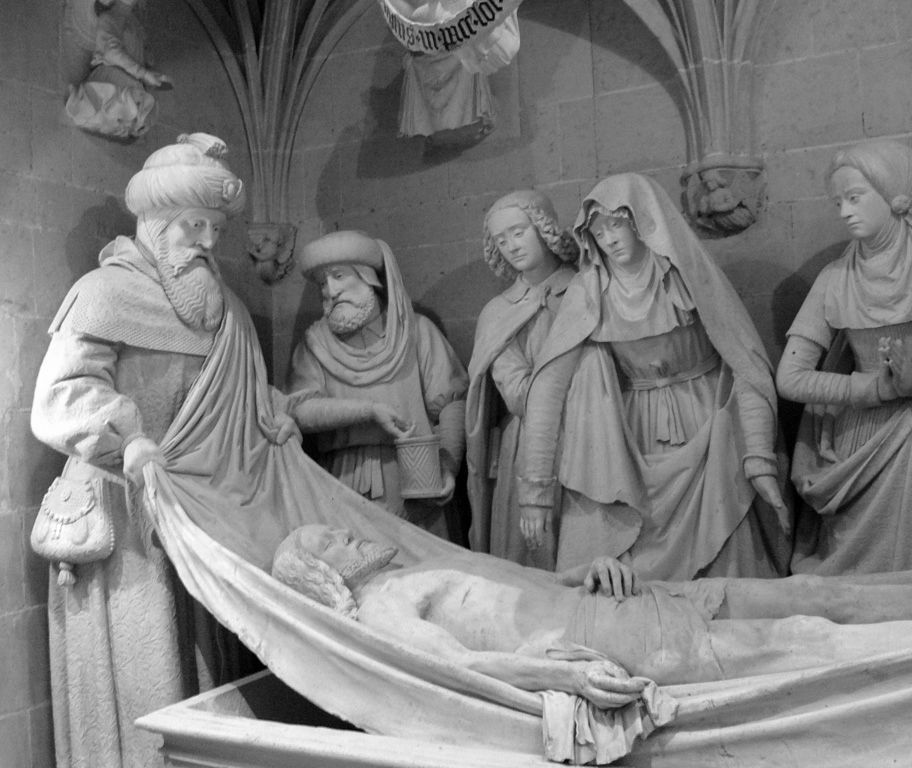
\includegraphics[width=8cm]{../commun/tombeau.png}

\renewcommand{\textheight}{10cm}

\vspace*{1cm}

\begin{Huge}
LATIN - FRANÇAIS
\end{Huge}

\vspace*{1cm}

\begin{huge}
Schola Saint-Maur
\end{huge}

\end{center}
\endgroup

\newpage
\newpage

\end{titlepage}

% Premier nocturne



\fancyhead[CO]{\bfseries \uppercase{Samedi Saint - Premier nocturne}}

\titrenocturne{Premier nocturne.}

\rubrique{On ne chante ni invitatoire, ni hymne, mais on commence directement
par la première antienne, en se signant les lèvres.}

\rubrique{A la fin de chaque psaume, un des servants éteint l’un des quinze cierges du chandelier
qui aura été placé en avant de l’autel.}

\ssmAnnotation{6mm}{1 \Abar. VIII g}
\ssmCommentary{-1mm}{Cf. Ps. 4, 9}
\nopagebreak
\includescore{../AM2005/ant_In_pace.tex}
\nopagebreak
\input{../commun/fr/ant_In_pace_fr}

% Psaume 4

\input{../ps/fr/tit_ps4_fr}
\input{../ps/neo-vulgate/int_ps4_8}
\input{../ps/neo-vulgate/ps4_8}

% Antienne 2

\ssmAnnotation{3mm}{2 \Abar. IV e}
\ssmCommentary{0mm}{Cf. Ps. 14, 1}
\nopagebreak
\includescore{../AM2005/ant_Habitabit.tex}
\nopagebreak
\input{../commun/fr/ant_Habitabit_fr}

% Psaume 14
\input{../ps/fr/tit_ps14_fr}
\input{../ps/neo-vulgate/int_ps14_4}
\input{../ps/neo-vulgate/ps14_4}

% Antienne 3

\ssmAnnotation{4mm}{3 \Abar. VII c}
\ssmCommentary{0mm}{Cf. Ps. 15, 9}
\nopagebreak
\includescore{../AM2005/ant_Caro_mea.tex}
\nopagebreak
\input{../commun/fr/ant_Caro_mea_fr}

% Psaume 15
\input{../ps/fr/tit_ps15_fr}
\input{../ps/neo-vulgate/int_ps15_7_transp}
\input{../ps/neo-vulgate/ps15_7}

\rubriquefinpsaumes

\ssmCommentary{0mm}{Cf. Ps. 21, 19}
\nopagebreak
\includescore{../commun/vers_In_pace_in_idipsum.tex}
\nopagebreak
\input{../commun/fr/vers_In_pace_in_idipsum_fr}

\rubriquefinverset

% Leçon I

\titrelecture{Lecture I.}
\nopagebreak
\reflect{Lect_I}
\nopagebreak
\input{../lect/lt/lect_I_lt}

% Répons I

\ssmCommentary{0mm}{Cf. Mt. 27, 62\,.\,67}
\nopagebreak
\ssmAnnotation{4mm}{1 \Rbar. II}
\includescore{../AM2005/resp_Sepulto.tex}
\nopagebreak
\input{../commun/fr/resp_Sepulto_fr}

% Leçon II

\titrelecture{Lecture II.}
\nopagebreak
\reflect{Lect_II}
\nopagebreak
\input{../lect/lt/lect_II_lt}

% Répons II

\ssmAnnotation{4mm}{2 \Rbar. V}
\includescore{../AM2005/resp_Ierusalem.tex}
\nopagebreak
\input{../commun/fr/resp_Ierusalem_fr}

% Leçon III
\titrelecture{Lecture III.}
\nopagebreak
\reflect{Lect_III}
\nopagebreak
\input{../lect/lt/lect_III_lt}

% Répons III
\ssmCommentary{0mm}{Cf. Mt. 26, 38\,.\,45}
\nopagebreak
\ssmAnnotation{4mm}{3 \Rbar. V}
\includescore{../AM2005/resp_Plange.tex}
\nopagebreak
\input{../commun/fr/resp_Plange_fr}

\rubrique{On garde le silence un instant. Au signal du cérémoniaire, tous se lèvent,
 et on entonne la première antienne du deuxième nocturne.}


\finnocturne
% Deuxième nocturne

\newpage

\fancyhead[CO]{\bfseries \uppercase{Samedi Saint - Deuxième nocturne}}

\titrenocturne{Deuxième nocturne.}

% Antienne 1

\ssmAnnotation{5mm}{1 \Abar. V a}
\ssmCommentary{0mm}{Cf. Ps. 23, 9}
\nopagebreak
\includescore{../AM2005/ant_Elevamini.tex}
\nopagebreak
\input{../commun/fr/ant_Elevamini_fr}

% Psaume 23
\input{../ps/fr/tit_ps23_fr}
\input{../ps/neo-vulgate/int_ps23_5}
\input{../ps/neo-vulgate/ps23_5}

% Antienne 2

\ssmAnnotation{5mm}{2 \Abar. IV e}
\ssmCommentary{0mm}{Cf. Ps. 26, 13}
\nopagebreak
\includescore{../AM2005/ant_Credo_videre.tex}
\nopagebreak
\input{../commun/fr/ant_Credo_videre_fr}

% Psaume 26
\input{../ps/fr/tit_ps26_fr}
\input{../ps/neo-vulgate/int_ps26_4}
\input{../ps/neo-vulgate/ps26_4}

% Antienne 3

\ssmAnnotation{5mm}{3 \Abar. VIII g}
\ssmCommentary{0mm}{Cf. Ps. 29, 4}
\nopagebreak
\includescore{../AM2005/ant_Domine_abstraxisti.tex}
\nopagebreak
\input{../commun/fr/ant_Domine_abstraxisti_fr}

% Psaume 29
\input{../ps/fr/tit_ps29_fr}
\input{../ps/neo-vulgate/int_ps29_8}
\input{../ps/neo-vulgate/ps29_8}

\rubriquefinpsaumes

% Verset

\ssmCommentary{0mm}{Cf. Ps. 40, 11}
\nopagebreak
\includescore{../commun/vers_Tu_autem.tex}
\nopagebreak
\input{../commun/fr/vers_Tu_autem_fr}

\rubriquefinverset

% Leçon IV
\titrelecture{Lecture IV.}
\nopagebreak
\reflect{Lect_IV}
\nopagebreak
\input{../lect/LH/lt/lect_IV_lt}

% Répons IV

\ssmAnnotation{5mm}{4 \Rbar. VII}
\includescore{../AM2005/resp_Recessit.tex}
\nopagebreak
\input{../commun/fr/resp_Recessit_fr}

% Leçon V
\titrelecture{Lecture V.}
\nopagebreak
\reflect{Lect_V}
\nopagebreak
\input{../lect/LH/lt/lect_V_lt}

% Répons V

\ssmCommentary{+1mm}{Cf. Mt. 26, 55}
\nopagebreak
\ssmAnnotation{5mm}{5 \Rbar. VIII}
\includescore{../AM2005/resp_O_vos_omnes.tex}
\nopagebreak
\input{../commun/fr/resp_O_vos_omnes_fr}

% Leçon VI
\titrelecture{Lecture VI.}
\nopagebreak
\reflect{Lect_VI}
\nopagebreak
\input{../lect/LH/lt/lect_VI_lt}

% Répons VI
\ssmCommentary{-1mm}{Cf. Is. 57, 1; 53, 7-8}
\nopagebreak
\ssmAnnotation{5mm}{6 \Rbar. IV}
\includescore{../AM2005/resp_Ecce.tex}
\nopagebreak
\input{../commun/fr/resp_Ecce_fr}

\rubrique{On garde le silence un instant. Au signal du cérémoniaire, tous se lèvent,
 et on entonne la première antienne du troisième nocturne.}

\finnocturne

% Troisième nocturne

\newpage

\fancyhead[CO]{\bfseries \uppercase{Samedi Saint - Troisième nocturne}}

\titrenocturne{Troisième nocturne.}

% Antienne 1

\ssmAnnotation{5mm}{1 \Abar. VIII g}
\ssmCommentary{-1mm}{Cf. Ps. 53, 6}
\nopagebreak
\includescore{../AM2005/ant_Deus_adiuvat_me.tex}
\nopagebreak
\input{../commun/fr/ant_Deus_adiuvat_me_fr}

% Psaume 53
\input{../ps/fr/tit_ps53_fr}
\input{../ps/neo-vulgate/int_ps53_8}
\input{../ps/neo-vulgate/ps53_8}

% Antienne 2

\ssmAnnotation{5mm}{2 \Abar. VII a}
\ssmCommentary{1mm}{Cf. Ps. 75, 3}
\nopagebreak
\includescore{../AM2005/ant_In_pace_factus_est.tex}
\nopagebreak
\input{../commun/fr/ant_In_pace_factus_est_fr}

% Psaume 75
\input{../ps/fr/tit_ps75_fr}
\input{../ps/neo-vulgate/int_ps75_7}
\input{../ps/neo-vulgate/ps75_7}

% Antienne 3

\ssmAnnotation{5mm}{3 \Abar. IV d}
\ssmCommentary{0mm}{Cf. Ps. 87, 5-6}
\nopagebreak
\includescore{../AM2005/ant_Factus_sum.tex}
\nopagebreak
\input{../commun/fr/ant_Factus_sum_fr}

% Psaume 87
\input{../ps/fr/tit_ps87_fr}
\input{../ps/neo-vulgate/int_ps87_4}
\input{../ps/neo-vulgate/ps87_4}

\rubriquefinpsaumes

% Verset
\ssmCommentary{0mm}{Cf. Ps. 75, 3}
\nopagebreak
\includescore{../commun/vers_In_pace_factus_est.tex}
\nopagebreak
\input{../commun/fr/vers_In_pace_factus_est_fr}

\rubriquefinverset

% Leçon VII
\titrelecture{Lecture VII.}
\nopagebreak
\reflect{Lect_VII}
\nopagebreak
\input{../lect/LH/lt/lect_VII_lt}

% Répons VII

\ssmCommentary{-1mm}{Cf. Ps. 87, 5\,.\,6\,.\,7}
\nopagebreak
\ssmAnnotation{5mm}{7 \Rbar. IV}
\includescore{../AM2005/resp_Aestimatus_sum.tex}
\nopagebreak
\input{../commun/fr/resp_Aestimatus_sum_fr}

% Leçon VIII
\titrelecture{Lecture VIII.}
\nopagebreak
\reflect{Lect_VIII}
\nopagebreak
\input{../lect/LH/lt/lect_VIII_lt}

% Répons VIII
\ssmCommentary{0mm}{Cf. Ps. 2, 2\,.\,1}
\nopagebreak
\ssmAnnotation{5mm}{8 \Rbar. IV}
\includescore{../AM2005/resp_Astiterunt.tex}
\nopagebreak
\input{../commun/fr/resp_Astiterunt_fr}

% Leçon IX
\titrelecture{Lecture IX.}
\nopagebreak
\reflect{Lect_IX}
\nopagebreak
\input{../lect/LH/lt/lect_IX_lt}

% Répons IX

\ssmCommentary{0mm}{Cf. Mt. 27, 62\,.\,67}
\nopagebreak
\ssmAnnotation{5mm}{9 \Rbar. IV}
\includescore{../AM2005/resp_Sicut_ovis.tex}
\nopagebreak
\input{../commun/fr/resp_Sicut_ovis_fr}

\rubrique{On garde le silence un instant. Au signal du cérémoniaire, tous se lèvent et se
tournent vers l’autel. L’officiant entonne la première antienne des Laudes, et tous se
signent.}

\finnocturne

% Laudes

\newpage

\fancyhead[CO]{\bfseries \uppercase{Samedi Saint - Laudes}}

\titrelaudes{Laudes}

% Antienne 1

\ssmAnnotation{5mm}{1 \Abar. II* d}
\ssmCommentary{0mm}{Cf. Rom 8, 32}
\nopagebreak
\includescore{../AM2005/ant_O_mors.tex}
\nopagebreak
\input{../commun/fr/ant_O_mors_fr}

% Psaume 50
\input{../ps/fr/tit_ps50_fr}
\input{../ps/neo-vulgate/int_ps50_2_etoile}
\input{../ps/neo-vulgate/ps50_2_etoile}

% Antienne 2

\ssmAnnotation{5mm}{2 \Abar. II* a}
\ssmCommentary{1mm}{Cf. Za 12, 10}
\nopagebreak
\includescore{../AM2005/ant_Plangent_eum.tex}
\nopagebreak
\input{../commun/fr/ant_Plangent_eum_fr}

% Psaume 91
\input{../ps/fr/tit_ps91_fr}
\input{../ps/neo-vulgate/int_ps91_2_etoile}
\input{../ps/neo-vulgate/ps91_2_etoile}

% Antienne 3

\ssmAnnotation{5mm}{3 \Abar. VII b}
\ssmCommentary{0mm}{Cf. Lm 1, 18}
\nopagebreak
\includescore{../AM2005/ant_Attendite.tex}
\nopagebreak
\input{../commun/fr/ant_Attendite_fr}

% Psaume 63
\input{../ps/fr/tit_ps63_fr}
\input{../ps/neo-vulgate/int_ps63_7}
\input{../ps/neo-vulgate/ps63_7}

% Antienne 4

\ssmAnnotation{5mm}{4 \Abar. II d}
\includescore{../AM2005/ant_A_porta_inferi.tex}
\nopagebreak
\input{../commun/fr/ant_A_porta_inferi_fr}

% Psaume AT23
\input{../ps/fr/tit_at23_fr}
\input{../ps/neo-vulgate/int_at23_2}
\input{../ps/neo-vulgate/at23_2}

% Antienne 5

\ssmAnnotation{5mm}{5 \Abar. VIII c}
\ssmCommentary{+1mm}{Cf. Lm 1, 12}
\nopagebreak
\includescore{../AM2005/ant_O_vos_omnes.tex}
\nopagebreak
\input{../commun/fr/ant_O_vos_omnes_fr}

% Psaume 150
\input{../ps/fr/tit_ps150_fr}
\input{../ps/neo-vulgate/int_ps150_8}
\input{../ps/neo-vulgate/ps150_8}

\textcolor{red}{\itshape On ne dit pas de Lecture Brève, mais au signal du
cérémoniaire, tous se lèvent et, tournés vers l’autel, répondent au verset
proclamé par un chantre. L’officiant entonne alors l’antienne du} Benedíctus.

% Verset
\ssmCommentary{-1mm}{Cf. Ps. 15, 9\,.\,10}
\nopagebreak
\includescore{../commun/vers_Caro_mea.tex}
\nopagebreak
\input{../commun/fr/vers_Caro_mea_fr}

% Antienne du Benedictus

\ssmAnnotation{5mm}{\Abar. I g}
\includescore{../AM2005/ant_Mulieres.tex}
\nopagebreak
\input{../commun/fr/ant_Mulieres_fr}

% Benedictus
\begin{center}
\uppercase{\Large{Benedictus}}
\end{center}
\nopagebreak
\ssmCommentary{-1mm}{Cf. Lc 1, 68-79}
\nopagebreak
\input{../ps/neo-vulgate/int_benedictus_1}
\nopagebreak
\input{../ps/neo-vulgate/benedictus_1}

\textcolor{red}{\itshape Les cierges du chandelier triangulaire ont été
successivement éteints. Un seul, placé au sommet du chandelier, est resté allumé.
Pendant le} Benedíctus, \textcolor{red}{\itshape on éteint les six cierges qui
brûlent sur l’autel, de chaque côté alternativement, de manière que tous soient
éteints au dernier verset. On éteint aussi toutes les lumières de l’église.}

\textcolor{red}{\itshape Après la reprise de l’antienne} Mulíeres, %
\textcolor{red}{\itshape tous se mettent à genoux et chantent le Christus, %
pendant lequel un des servants retire le cierge resté allumé, et va le dissimuler
derrière l’autel.}

\ssmAnnotation{5mm}{\Abar.}
\ssmCommentary{1mm}{Cf. Phil 2,8-9}
\nopagebreak
\includescore{../AM2005/ant_Christus.tex}
\nopagebreak
\input{../commun/fr/ant_Christus_fr}

\textcolor{red}{\itshape On garde le silence le temps d’un} Notre Père. %
\textcolor{red}{\itshape L’officiant lit alors l’oraison sans dire} Orémus, %
\textcolor{red}{\itshape sur un ton assez grave, en descendant d’un ton sur
la dernière syllabe et sans conclusion.}

% Oraison

\begin{center}
\textbf{Oraison.}
\end{center}

\input{../commun/oratio}

\rubrique{L’oraison terminée, on frappe avec bruit sur les stalles, jusqu’à ce que le cierge resté
allumé soit déposé au sommet du chandelier. Au signal du cérémoniaire, tous se lèvent
alors et se retirent en silence.}


\finoffice

% Annexes
\newpage

\fancyhead[CO]{\bfseries \uppercase{Samedi Saint - Annexes}}

\begin{appendices}

\label{Lect_I}
\titrelecture{Lecture I.}
\includescore{../lect/lect_I.tex}

\newpage
\label{Lect_II}
\titrelecture{Lecture II.}
\includescore{../lect/lect_II.tex}

\newpage
\label{Lect_III}
\titrelecture{Lecture III.}
\includescore{../lect/lect_III.tex}

\newpage
\label{Lect_IV}
\titrelecture{Lecture IV.}
\includescore{../lect/LH/lect_IV.tex}

\newpage
\label{Lect_V}
\titrelecture{Lecture V.}
\includescore{../lect/LH/lect_V.tex}

\newpage
\label{Lect_VI}
\titrelecture{Lecture VI.}
\includescore{../lect/LH/lect_VI.tex}

\newpage
\label{Lect_VII}
\titrelecture{Lecture VII.}
\includescore{../lect/LH/lect_VII.tex}

\newpage
\label{Lect_VIII}
\titrelecture{Lecture VIII.}
\includescore{../lect/LH/lect_VIII.tex}

\newpage
\label{Lect_IX}
\titrelecture{Lecture IX.}
\includescore{../lect/LH/lect_IX.tex}

\end{appendices}

% Index

%\newpage

%\tableofcontents

\end{document}
